\documentclass[tikz,border=6pt]{standalone}
\usepackage{amsmath,amssymb}
\usetikzlibrary{arrows.meta, positioning, calc, backgrounds, fit}

\definecolor{nodeblue}{HTML}{2C5FAA}
\definecolor{nodefill}{HTML}{EAF1FA}
\definecolor{multi}{HTML}{B03A2E}
\definecolor{multifill}{HTML}{FDEDEC}
\definecolor{bandbg}{HTML}{F8F8F8}
\definecolor{edgegray}{HTML}{4A4A4A}

\begin{document}

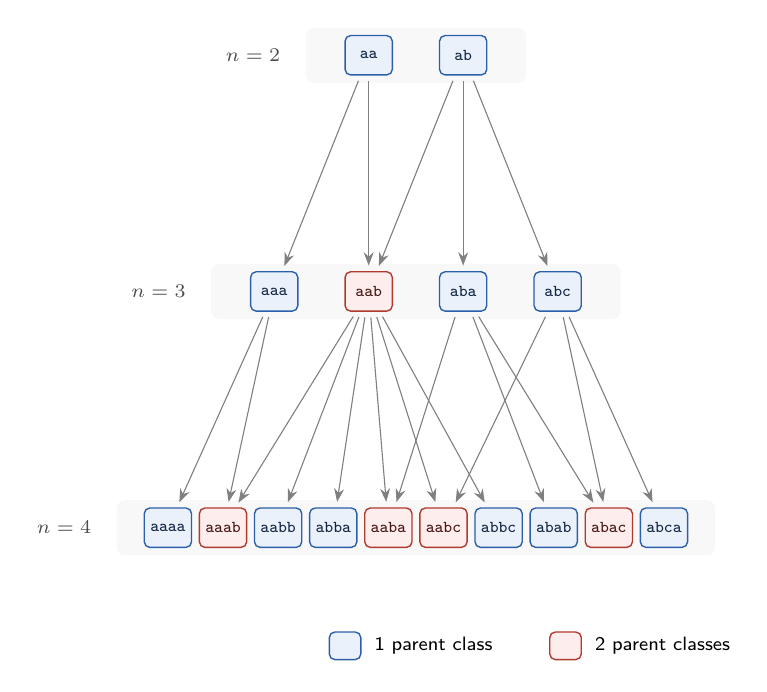
\begin{tikzpicture}[
    x=1cm, y=1cm,
    font=\footnotesize,
    >=Stealth,
    dag node/.style={
        rounded corners=2pt,
        draw=nodeblue,
        fill=nodefill,
        line width=0.5pt,
        minimum width=6mm,
        minimum height=5mm,
        inner sep=0pt,
        font=\fontsize{6}{7}\selectfont\ttfamily,
        text=nodeblue!40!black
    },
    multi node/.style={
        dag node,
        draw=multi,
        fill=multifill,
        text=multi!40!black
    },
    dag edge/.style={
        ->,
        draw=edgegray!70,
        line width=0.4pt,
        shorten >=2pt,
        shorten <=2pt
    },
    level label/.style={
        font=\scriptsize\sffamily\bfseries\color{gray!60!black},
        anchor=east
    }
]

% Bandas de fondo
\begin{scope}[on background layer]
    \fill[bandbg, rounded corners=3pt] (-1.4, 0.35) rectangle (1.4, -0.35);
    \fill[bandbg, rounded corners=3pt] (-2.6, -2.65) rectangle (2.6, -3.35);
    \fill[bandbg, rounded corners=3pt] (-3.8, -5.65) rectangle (3.8, -6.35);
\end{scope}

% Etiquetas de nivel
\node[level label] at (-1.6, 0) {$n=2$};
\node[level label] at (-2.8, -3.0) {$n=3$};
\node[level label] at (-4.0, -6.0) {$n=4$};

% Nivel n=2
\node[dag node] (aa) at (-0.6, 0) {aa};
\node[dag node] (ab) at ( 0.6, 0) {ab};

% Nivel n=3
\node[dag node]   (aaa) at (-1.8, -3.0) {aaa};
\node[multi node] (aab) at (-0.6, -3.0) {aab};
\node[dag node]   (aba) at ( 0.6, -3.0) {aba};
\node[dag node]   (abc) at ( 1.8, -3.0) {abc};

% Nivel n=4 (orden elegido para minimizar cruces)
\node[dag node]   (aaaa) at (-3.15, -6.0) {aaaa};
\node[multi node] (aaab) at (-2.45, -6.0) {aaab};
\node[dag node]   (aabb) at (-1.75, -6.0) {aabb};
\node[dag node]   (abba) at (-1.05, -6.0) {abba};
\node[multi node] (aaba) at (-0.35, -6.0) {aaba};
\node[multi node] (aabc) at ( 0.35, -6.0) {aabc};
\node[dag node]   (abbc) at ( 1.05, -6.0) {abbc};
\node[dag node]   (abab) at ( 1.75, -6.0) {abab};
\node[multi node] (abac) at ( 2.45, -6.0) {abac};
\node[dag node]   (abca) at ( 3.15, -6.0) {abca};

% Aristas n=2 → n=3
\draw[dag edge] (aa) -- (aaa);
\draw[dag edge] (aa) -- (aab);
\draw[dag edge] (ab) -- (aab);
\draw[dag edge] (ab) -- (aba);
\draw[dag edge] (ab) -- (abc);

% Aristas n=3 → n=4
\draw[dag edge] (aaa) -- (aaaa);
\draw[dag edge] (aaa) -- (aaab);
\draw[dag edge] (aab) -- (aaab);
\draw[dag edge] (aab) -- (aabb);
\draw[dag edge] (aab) -- (abba);
\draw[dag edge] (aab) -- (aaba);
\draw[dag edge] (aab) -- (aabc);
\draw[dag edge] (aab) -- (abbc);
\draw[dag edge] (aba) -- (aaba);
\draw[dag edge] (aba) -- (abab);
\draw[dag edge] (aba) -- (abac);
\draw[dag edge] (abc) -- (aabc);
\draw[dag edge] (abc) -- (abac);
\draw[dag edge] (abc) -- (abca);

% Leyenda horizontal debajo
\begin{scope}[shift={(0, -7.5)}]
    \node[dag node, minimum width=4mm, minimum height=3.5mm,
          font=\tiny] at (-0.9, 0) {};
    \node[anchor=west, font=\scriptsize\sffamily] at (-0.65, 0) {1 parent class};
    \node[multi node, minimum width=4mm, minimum height=3.5mm,
          font=\tiny] at (1.9, 0) {};
    \node[anchor=west, font=\scriptsize\sffamily] at (2.15, 0) {2 parent classes};
\end{scope}

\end{tikzpicture}
\end{document}
